\documentclass[tikz,border=6pt]{standalone}
\usepackage{amsmath}
\usetikzlibrary{arrows.meta,calc,positioning}

\begin{document}

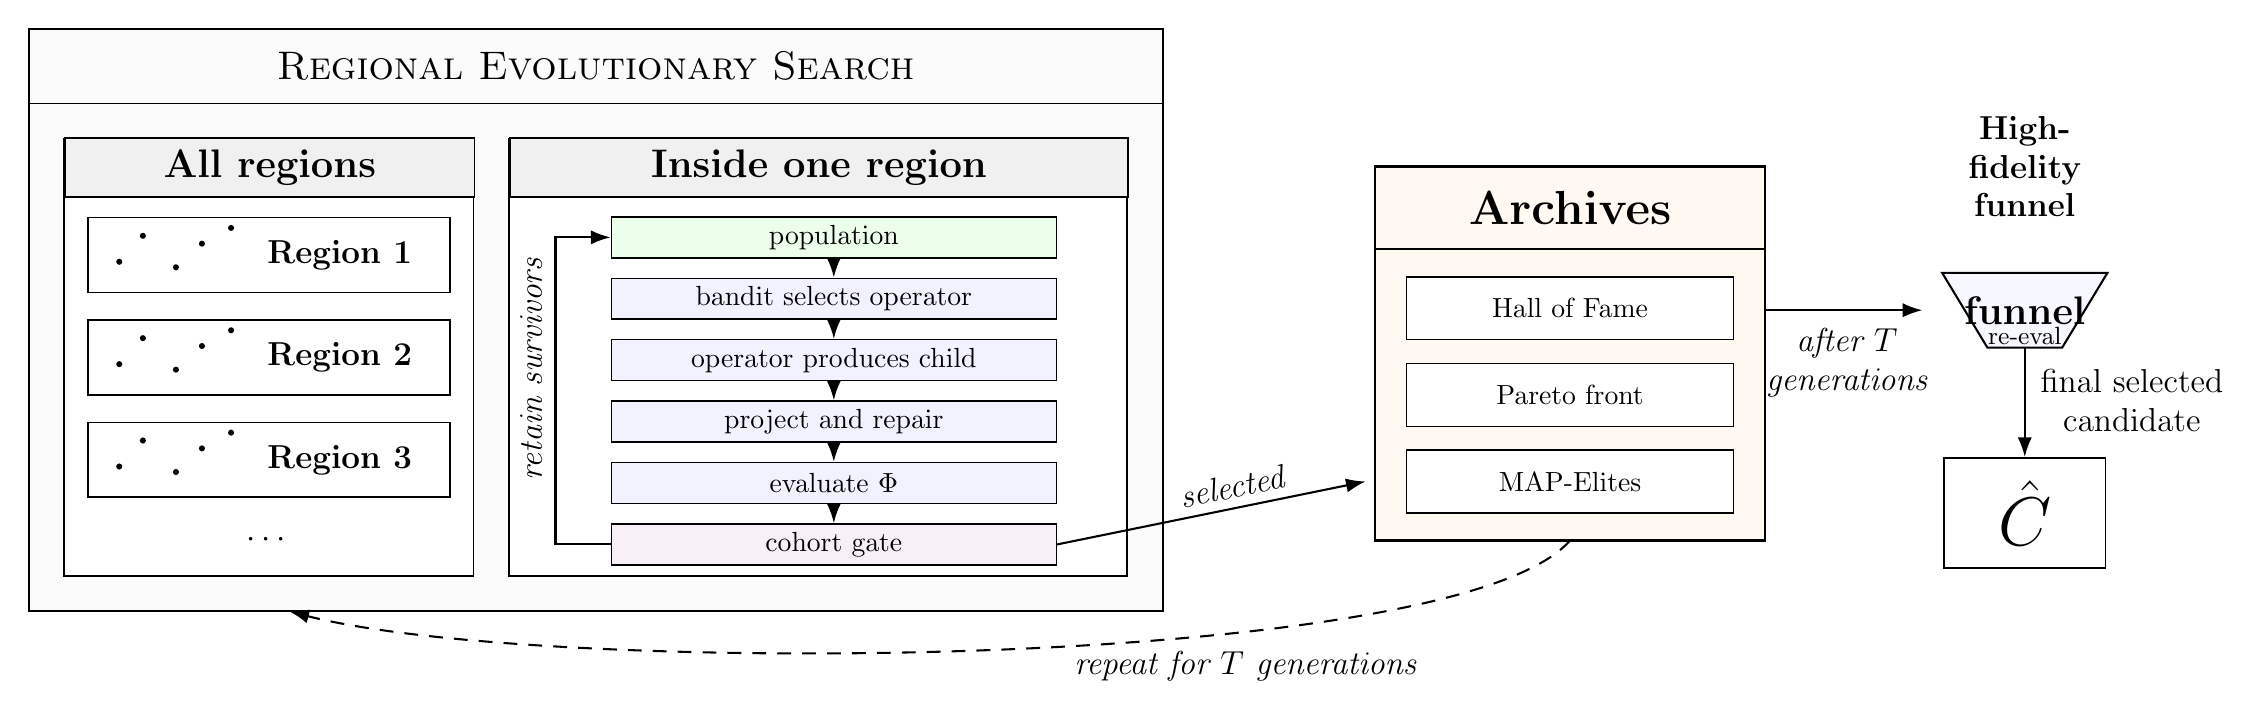
\begin{tikzpicture}[
  x=1cm,y=1cm,
  font=\sffamily,
  >={Latex[length=2.5mm,width=1.8mm]},
  outer/.style={draw=black,line width=0.75pt,fill=gray!3},
  panel/.style={draw=black,line width=0.65pt,fill=white},
  header/.style={
    draw=black,
    line width=0.65pt,
    fill=gray!12,
    font=\bfseries\Large,
    align=center
  },
  title/.style={
    font=\Large\scshape,
    align=center
  },
  box/.style={
    draw=black,
    line width=0.55pt,
    fill=white,
    align=center,
    font=\normalsize,
    inner sep=2pt
  },
  flow/.style={box,minimum height=0.52cm},
  lab/.style={font=\large\itshape},
  dot/.style={
    circle,
    fill=black,
    inner sep=0pt,
    minimum size=2.2pt
  },
  arr/.style={->,line width=0.75pt},
  darr/.style={
    ->,
    line width=0.75pt,
    dashed,
    dash pattern=on 5pt off 4pt
  }
]

% ============================================================
% Calculated layout dimensions, in centimetres
% ============================================================

\pgfmathsetmacro{\Lx}{0}
\pgfmathsetmacro{\Ly}{0}
\pgfmathsetmacro{\LW}{14.40}
\pgfmathsetmacro{\LH}{7.40}

\pgfmathsetmacro{\TitleH}{0.95}
\pgfmathsetmacro{\Pad}{0.45}
\pgfmathsetmacro{\Gap}{0.45}

\pgfmathsetmacro{\AllW}{5.20}
\pgfmathsetmacro{\InW}{\LW-2*\Pad-\Gap-\AllW}

\pgfmathsetmacro{\AllX}{\Lx+\Pad}
\pgfmathsetmacro{\InX}{\AllX+\AllW+\Gap}

\pgfmathsetmacro{\ColY}{\Ly+\Pad}
\pgfmathsetmacro{\ColH}{\LH-\TitleH-2*\Pad}
\pgfmathsetmacro{\ColTop}{\ColY+\ColH}

\pgfmathsetmacro{\HdrH}{0.75}
\pgfmathsetmacro{\BodyTop}{\ColTop-\HdrH}
\pgfmathsetmacro{\TitleSepY}{\Ly+\LH-\TitleH}

% ============================================================
% Main search container
% ============================================================

\draw[outer] (\Lx,\Ly) rectangle ++(\LW,\LH);
\draw[line width=0.65pt] (\Lx,\TitleSepY) -- ++(\LW,0);

\node[title] at ({\Lx+\LW/2},{\TitleSepY+\TitleH/2})
{Regional Evolutionary Search};

% ============================================================
% Left two panels
% ============================================================

\draw[panel] (\AllX,\ColY) rectangle ++(\AllW,\ColH);

\node[
  header,
  minimum width=\AllW cm,
  minimum height=\HdrH cm,
  anchor=south west
] at (\AllX,\BodyTop) {All regions};

\draw[panel] (\InX,\ColY) rectangle ++(\InW,\ColH);

\node[
  header,
  minimum width=\InW cm,
  minimum height=\HdrH cm,
  anchor=south west
] at (\InX,\BodyTop) {Inside one region};

% ============================================================
% Region boxes
% ============================================================

\pgfmathsetmacro{\RegW}{\AllW-0.60}
\pgfmathsetmacro{\RegH}{0.95}
\pgfmathsetmacro{\RegX}{\AllX+0.30}
\pgfmathsetmacro{\RegCTextX}{\RegX+3.20}

\foreach \yy/\num in {4.05/1,2.75/2,1.45/3}{
  \draw[box] (\RegX,\yy) rectangle ++(\RegW,\RegH);

  \begin{scope}[shift={({\RegX+0.40},{\yy+0.27})}]
    \node[dot] at (0.00,0.12) {};
    \node[dot] at (0.30,0.45) {};
    \node[dot] at (0.72,0.05) {};
    \node[dot] at (1.05,0.35) {};
    \node[dot] at (1.42,0.55) {};
  \end{scope}

  \node[font=\bfseries\large] at
  (\RegCTextX,{\yy+\RegH/2}) {Region \num};
}

\node[font=\large] at ({\AllX+\AllW/2},{\ColY+0.45}) {$\cdots$};

% ============================================================
% Inside-region pipeline
% ============================================================

\pgfmathsetmacro{\FlowW}{\InW-2.20}
\pgfmathsetmacro{\FlowX}{\InX+1.30}
\pgfmathsetmacro{\FlowCX}{\FlowX+\FlowW/2}

\pgfmathsetmacro{\FlowH}{0.52}
\pgfmathsetmacro{\Step}{0.78}
\pgfmathsetmacro{\Yone}{\BodyTop-0.50}

\node[
  flow,
  fill=green!8,
  minimum width=\FlowW cm
] (population) at (\FlowCX,\Yone) {population};

\node[
  flow,
  fill=blue!5,
  minimum width=\FlowW cm
] (bandit) at (\FlowCX,{\Yone-\Step}) {bandit selects operator};

\node[
  flow,
  fill=blue!5,
  minimum width=\FlowW cm
] (operator) at (\FlowCX,{\Yone-2*\Step}) {operator produces child};

\node[
  flow,
  fill=blue!5,
  minimum width=\FlowW cm
] (repair) at (\FlowCX,{\Yone-3*\Step}) {project and repair};

\node[
  flow,
  fill=blue!5,
  minimum width=\FlowW cm
] (eval) at (\FlowCX,{\Yone-4*\Step}) {evaluate $\Phi$};

\node[
  flow,
  fill=violet!6,
  minimum width=\FlowW cm
] (cohort) at (\FlowCX,{\Yone-5*\Step}) {cohort gate};

\draw[arr] (population.south) -- (bandit.north);
\draw[arr] (bandit.south) -- (operator.north);
\draw[arr] (operator.south) -- (repair.north);
\draw[arr] (repair.south) -- (eval.north);
\draw[arr] (eval.south) -- (cohort.north);

% Survivor loop, routed outside the boxes.
\draw[arr] (cohort.west) -- ++(-0.70,0) |- (population.west);

\node[lab,rotate=90] at
({\InX+0.28},{\ColY+\ColH/2-0.15})
{retain survivors};

% ============================================================
% Archives block
% ============================================================

\pgfmathsetmacro{\ArcX}{\Lx+\LW+2.70}
\pgfmathsetmacro{\ArcY}{0.90}
\pgfmathsetmacro{\ArcW}{4.95}
\pgfmathsetmacro{\ArcH}{4.75}

\pgfmathsetmacro{\ArcTitleH}{1.05}
\pgfmathsetmacro{\ArcTop}{\ArcY+\ArcH}
\pgfmathsetmacro{\ArcTitleSep}{\ArcTop-\ArcTitleH}

\draw[outer,fill=orange!5] (\ArcX,\ArcY) rectangle ++(\ArcW,\ArcH);
\draw[line width=0.65pt] (\ArcX,\ArcTitleSep) -- ++(\ArcW,0);

\node[font=\bfseries\LARGE] at
({\ArcX+\ArcW/2},{\ArcTitleSep+\ArcTitleH/2})
{Archives};

\pgfmathsetmacro{\AboxW}{\ArcW-0.80}

\node[
  box,
  minimum width=\AboxW cm,
  minimum height=0.80cm
] (hof) at
({\ArcX+\ArcW/2},{\ArcTitleSep-0.75})
{Hall of Fame};

\node[
  box,
  minimum width=\AboxW cm,
  minimum height=0.80cm
] (pareto) at
({\ArcX+\ArcW/2},{\ArcTitleSep-1.85})
{Pareto front};

\node[
  box,
  minimum width=\AboxW cm,
  minimum height=0.80cm
] (map) at
({\ArcX+\ArcW/2},{\ArcTitleSep-2.95})
{MAP-Elites};

% West edge of the outer Archives box, aligned vertically with MAP-Elites
\path let \p1 = (map.west) in
  coordinate (archiveWest) at ({\ArcX-0.12},\y1);

% Selected candidate path
\draw[arr]
  (cohort.east) --
  node[lab,above,sloped,pos=0.58] {selected}
  (archiveWest);

% Dashed repeat loop, deliberately routed below everything.
\draw[darr]
({\ArcX+\ArcW/2},{\ArcY})
.. controls ({\ArcX+1.0},-0.78)
and ({\Lx+\LW*0.45},-0.82)
.. ({\AllX+\AllW*0.55},{\Ly});

\node[lab] at
({(\ArcX+\Lx+\LW)/2-0.30},-0.70)
{repeat for $T$ generations};

% ============================================================
% High-fidelity funnel
% ============================================================

\pgfmathsetmacro{\FunX}{\ArcX+\ArcW+2.25}
\pgfmathsetmacro{\FunY}{3.35}
\pgfmathsetmacro{\FunTopW}{2.10}
\pgfmathsetmacro{\FunBotW}{0.95}
\pgfmathsetmacro{\FunH}{0.95}

\pgfmathsetmacro{\FunCX}{\FunX+\FunTopW/2}
\pgfmathsetmacro{\FunCY}{\FunY+\FunH/2}

\coordinate (funTopL) at (\FunX,{\FunY+\FunH});
\coordinate (funTopR) at ({\FunX+\FunTopW},{\FunY+\FunH});
\coordinate (funBotR) at ({\FunX+(\FunTopW+\FunBotW)/2},\FunY);
\coordinate (funBotL) at ({\FunX+(\FunTopW-\FunBotW)/2},\FunY);

\draw[
  draw=black,
  line width=0.75pt,
  fill=blue!3
]
(funTopL) -- (funTopR) -- (funBotR) -- (funBotL) -- cycle;

\node[font=\bfseries\Large] at (\FunCX,\FunCY) {funnel};
\node[font=\small] at (\FunCX,{\FunY+0.15}) {re-eval};

\node[
  font=\bfseries\large,
  align=center
] at
(\FunCX,{\FunY+\FunH+1.35})
{High-\\fidelity\\funnel};

% Archives to funnel arrow.
\draw[arr]
({\ArcX+\ArcW},{\FunCY}) --
node[lab,below=3pt,pos=0.52,align=center]
{after $T$\\generations}
({\FunX-0.25},{\FunCY});

% ============================================================
% Final selected candidate
% ============================================================

\pgfmathsetmacro{\CandW}{2.05}
\pgfmathsetmacro{\CandH}{1.40}
\pgfmathsetmacro{\CandY}{0.55}

\node[
  box,
  minimum width=\CandW cm,
  minimum height=\CandH cm,
  font=\Huge
] (candidate) at
(\FunCX,{\CandY+\CandH/2})
{$\hat{C}$};

\draw[arr]
(\FunCX,\FunY) --
node[
  font=\large,
  align=center,
  right=2pt,
  pos=0.48
]
{final selected\\candidate}
(candidate.north);

\end{tikzpicture}

\end{document}
